%! Author = Adrian Helberg
%! Date = 21.09.2020

% Preamble
\documentclass[11pt]{article}
% Packages
\usepackage{ngerman}
\usepackage{amsmath}
\usepackage{url}
\usepackage{graphicx}
\usepackage{float}
\usepackage{enumitem,amssymb}
\newlist{todolist}{itemize}{2}
\setlist[todolist]{label=$\square$}
\usepackage{pifont}
\newcommand{\cmark}{\ding{51}}%
\newcommand{\xmark}{\ding{55}}%
\newcommand{\done}{\rlap{$\square$}{\raisebox{2pt}{\large\hspace{1pt}\cmark}}%
\hspace{-2.5pt}}
\newcommand{\wontfix}{\rlap{$\square$}{\large\hspace{1pt}\xmark}}

\title{\textbf{Exposé} zur Bachelorarbeit von Adrian Helberg bei Prof. Dr. Jenke}

% Document
\begin{document}
    \maketitle

    \section{Problemstellung}

    Effizientes Objektdesign und -modellierung sind entscheidende Kernkompetenzen in verschiedenen Bereichen der
    digitalen Welt.
    Da die Erstellung geometrischer Objekte unintuitiv ist und ein großes Maß an Erfahrung und Expertise
    erfordert, ist dieses stetig wachsende Feld für Neueinsteiger nur sehr schwer zu erschließen.
    Die Forschung liefert hierzu einige Arbeiten zu prozeduraler Modellierung, um digitale Inhalte schneller und
    automatisiert zu erstellen.
    Die Bachelorarbeit soll sich auf die Erkenntnisse einer Basisquelle~\cite{basisquelle} stützen und im
    dreidimensionalen Kontext die inverse prozedurale Modellierung von Verzweigungsstrukturen beschreiben.
    Das in der Basisquelle beschriebene System generiert zweidimensionale Objekte mit Verzweigungsstrukturen.
    Hierzu soll ein prototypische Implementierung zur Überführung des Algorithmus vom zweidimensionalen in den
    dreisimensionalen Raum implementiert werden.

    \newpage

    \subsection{Konzepte und Ideen}
    Im Folgenden wird auf die Methodik zum Ableiten eines L-Systems, das eine zweidimensionale Verzweigungsstrukturen
    repräsentiert der Basisquelle~\cite{basisquelle} eingegangen und Konzepte und eigene Lösungsansätze präsentiert.

    \begin{figure}[H]
       \centering
       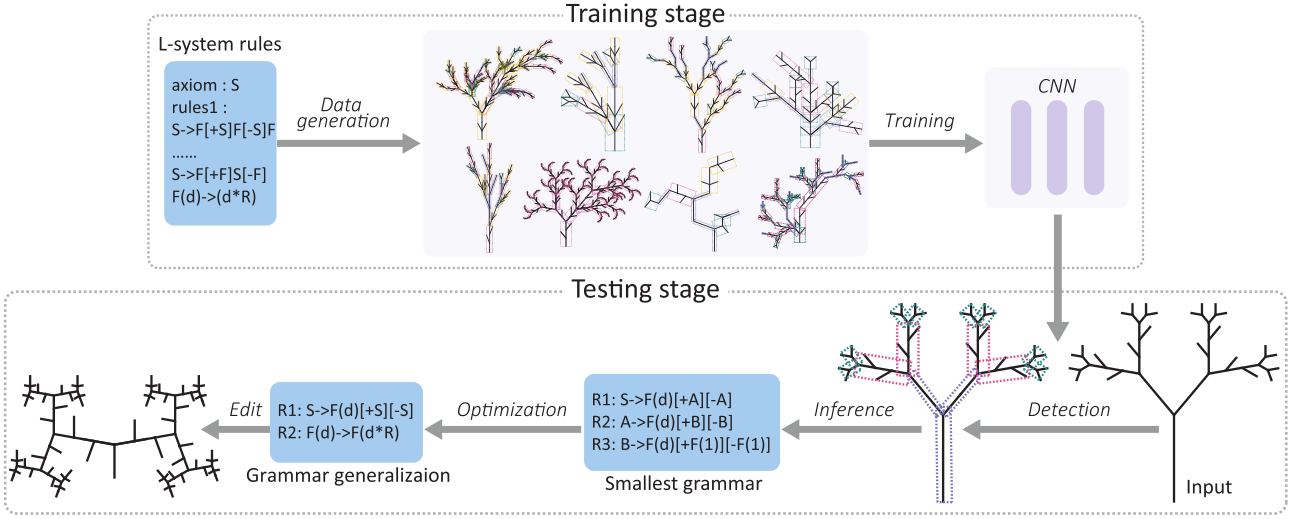
\includegraphics[width=14cm]{../images/System_2D.PNG}
       \caption[Systemarchitektur 2D]{Architektur des Systems der Basisquelle~\cite{basisquelle}}
    \end{figure}

    \subsubsection{System}
    Ziel des Systems ist die Erstellung von Ähnlichkeitsabbildern eines Input-Bildes.
    Hierzu wird eine beliebig verschachtelte Verzweigungsstruktur eingelesen, um eine Sammlung an ähnlichen Strukturen
    auszugeben.

    \subsubsection{Voraussetzungen}
    Das Input-Bild kann als Sammlung verschiedener, atomarer Stukturen\\(=\textbf{Templates}) gesehen werden, die mit
    diversen Parametern transformiert wurden.
    Um diese Strukturen zu erkennen, wird ein neuronales Netz anhand von generierten Trainingsdaten angelernt.
    Die Trainingsdaten werden anhand vordefinierter Templates, eines vordefinierten L-Systems und randomisierten
    Parametern generiert.\\
    Die in Input-Bildern erwarteten Verzweigungsstrukturen bilden die Templates, die jeweils an einen Schlüssel
    (=\textbf{Label}) gebunden sind.\\
    Um eine Zeichenkette, die Symbole eines L-Systems beinhaltet, zu visualisieren wird ein \textbf{Logo-Turtle-Algorithmus}
    genutzt~\cite{3}.

    \newpage

    \subsubsection{Überblick}
    \textit{Abbildung 1 zeigt, wie das o.g. System aufgebaut ist}:
    \begin{itemize}
        \item[I.] \underline{Training}: Ein neuronales Netz (\textbf{CNN}), das zur Erkennung von\\
        Verzweigungsstrukturen benötigt wird, wird trainiert.
        \begin{itemize}
            \item[a)] \textbf{Datengenerierung}: Mit dem vordefinierten L-System, einer zufälligen Auswahl an
            Templates und zufälligen Werten für Parameter werden Testdaten in Form von Bilden, die mit dem
            Logo-Turtle-Algorithmus gezeichnet werden, generiert.
            \item[b)] \textbf{Training}: Die generierten Bilder werden als Input in ein neuronales Netz gespeist
        \end{itemize}
        \item[II.] \underline{Testing}: Die Grammatik über Ähnlichkeitsabbilder des Input-Bildes wird abgeleitet.
        \begin{itemize}
            \item[a)] \textbf{Erkennung}: Das trainierte CNN ist in der Lage Strukturen eines unbekannten Input-Bildes
            zu erkennen und einem Schlüssel zuzuordnen
            \item[b)] \textbf{Inferenz}: Die erkannten Strukturen werden in einer Baumtopologie organisiert mit einem
            Startsymbol als Wurzelknoten, Terminalen als Knoten und Nicht-Terminalen als Blattknoten.
            Die Kanten des Baumes bilden die jeweils relative Transformation zum Elternknoten.
            Aus der Baumstruktur kann eine möglichst "`kleine"' Grammatik, die nur das Input-Bild beschreibt, abgeleitet
            werden.
            \item[c)] \textbf{Optimierung}: Die kompakte Grammatik wird um Rekursionen und nicht-deterministische
            Regeln erweitert, um ein L-System zu konstruieren, das nicht nur dem Input-Objekt entspricht, sondern
            eine größere Vielfalt repräsentiert.
            Anschließend werden ähnliche Regeln zu neuen Symbolen der Grammatik verbunden (\textbf{Generalisiserung}).
            \item[d)] \textbf{Bearbeitung}: Die Parameter der generalisierten Grammatik können vom Benutzer verändert
            werden, um das Ergebnis des Systems zu beeinflussen.
        \end{itemize}
    \end{itemize}

    \newpage

    \subsubsection{Umsetzung}
    \textit{Um das beschriebene System vom zweidimensionalen in den dreidimensionalen Raum zu überführen, sind einige
    Schritte nötig:}
    \begin{itemize}
        \item Das vordefinierte L-System muss Objekte im dreidimensionalen Raum erstellen
        \item Der Logo-Turtle-Algorithmus erhält eine weitere Dimension, um Objekte im 3D darstellen zu können.
        Derzeit gibt es eine 3D-Turtle-Grafik-Bibliothek~\cite{cheloniidae} für Java
        \item Die Struktur des neuronalen Netzes verändert sich, da sich die Trainingsdaten ändern.
        \item Evtl. sind "`Schnappschuss"'- Bilder des generierten 3D-Objektes aus verschiedenen Kameraperspektiven
        nötig, damit das CNN\\ Verzweigungsstrukturen im dreidimensionalen Raum erkennen kann~\cite{4}.
        \item Begrenzungskörper (\textbf{bounding boxes}), die als Schlüssel verwendet werden, müssen dreidimensional
        sein.
        \item Evtl. müssen Metriken zu Abstandsberechnung zweier Strukturen und heuristische Verfahren, wie der
        Greedy-Algorithmus zur Minimierung der Kostenfunktion bei der Generalisierung eines L-Systems,\\ dementsprechend
        angepasst werden
    \end{itemize}

    \subsection{Einführung}
    \textit{Die Einführung des Themas könnte wie folgt aussehen}:\\~\\
    Mit der Digitalisierung der Welt erlangt die Erstellung von digitalen Inhalten, wie 3D Modelle für Computerspiele,
    Webdesigns oder Visualisierung von Architektur, zunehmend an Bedeutung.
    Darum werden Verfahren gesucht, um Objekte dieser Felder formal zu beschreiben und somit kodifizierbar
    (\textit{engl. codify}) zu machen.
    Hierbei bilden sich folgende Klassen heraus:

    \newpage

    \begin{itemize}
        \item \textbf{Modellierung}: Um einen physikalischen Körper in ein digitales Objekt zu überführen, wird mithilfe
        von Abstraktion (oder Modellierung) ein mathematisches Modell erstellt, dass diesen Körper formal beschreibt.
        3D Grafiksoftware, wie Blender~\cite{blender}, wird genutzt um geometrische Körper zu modellieren, texturieren
        und zu animieren.
        \item \textbf{Prozedurale Modellierung}: \textit{"`It encompasses a wide variety of generative techniques that
        can (semi-−)automatically produce a specific type of content based on a set of input
        parameters."'}~\cite{1} \\
        "`Prozedurale Modellierung beschreibt generative Techniken, die \\(semi-)automatisch spezifische, digitale
        Inhalte anhand von deskriptiven Parametern erzeugen"' (\textit{Übersetzt durch den Autor})
        \item \textbf{Inverse prozedurale Modellierung (IPM)}:\textit{Aliaga et al.}~\cite{2}
        spricht bei der inversen prozeduralen Modellierung von dem Finden einer prozeduralen Repräsentation von
        Strukturen bestehender Modelle.
    \end{itemize}
    Die Modellierung mithilfe von Grafiksoftware ist eine vergleichbar händische, langwierige Erstellung von
    Objekten.
    Hierbei hat der Designer (= Modellierer) die volle Kontrolle über die Strukturen des Objektes.\\
    Bei der prozeduralen Modellierung werden spezifische Strukturen eines zu erstellenden physikalischen Objektes
    generalisiert und meist über eine Grammatik und globale Parameter abgebildet.
    Während bei der klassischen Modellierung die menschliche Intuition und bei der prozeduralen Modellierung eine
    parametrisierte Grammatik vorausgesetzt wird, arbeitet IPM mit bestehenden Modellen und extrahiert ("`lernt"')
    die Strukturen des Objektes, die automatisch in eine formale Grammatik überführt werden können.
    Die Generierung von prozeduralen Modellen ist ein wichtiges, offenes Problem~\cite{2}.\\
    Aktuelle Ansätze sind:
    \begin{itemize}
        \item Segmentierung von geometrischen Objekten in Ähnlichkeitsgruppen, um Muster (\textit{engl. Patterns}) zu
        erkennen und
        \item Kontrollierte Generierung durch Finden optimaler Prameter und Regeln
    \end{itemize}

    \newpage

    \subsection{Vorangehende Arbeiten}
    \textit{Dieses Kapitel beschreibt die relevanten Themen der Bachelorarbeit und stellt einige wissenenschaftliche
    Quellen vor:}
    \begin{itemize}
        \item (Inverse) Prozedurale Modellierung~\cite{2} und~\cite{1}:\\Siehe Kapitel 1.2 Einführung
        \item Logo-Turtle-Algorithmus~\cite{3}:\\ Der Logo-Turtle-Algorithmus bezeichnet eine Methode zur Generierung
        von Bildern mithilfe einer Zeichenkette, deren Symbole jeweils für einen bestimmten Befehl zur Steuerung einer
        "`Schildkröte"' (\textit{engl. turtle}) stehen.
        Die Visualisierung von Fraktalen und natürlicher Vegetation stellen zwei Beispiele für die Anwendung dar.
        \item \textbf{L-System}~\cite{5}:\\ L-Systeme sind spezielle, formale Grammatiken zur Beschreibung von
        natürlicher Vegetation.
        Lindenmayer führte dieses Stringersetzungssystem ein, um Zellteilung formal zu beschreiben.
        \item \textbf{Objekterkennung in Bildern}~\cite{6}:\\ In der zugehörigen Quelle wird das System "`DOTA"'
        beschrieben, das Objekte in Bildern mithilfe von bounding boxes erkennt und klassifiziert. Die Basisquelle~\cite{basisquelle}
        nutzt ebenfalls diesen Ansatz zur Objekterkennung.
        Trainingsdaten in Form von Bildern, in denen die zu erkennenden Formen mit Boxen vormarkiert sind, werden in
        ein neuronales Netz gespeist.
        Das CNN ist dann in der Lage Objekte in unbekannten Bilder zu erkennen und mit Boxen zu versehen.
    \end{itemize}

    \newpage

    \begin{itemize}

    \end{itemize}

    \section{Ablauf}
    \begin{itemize}
        \item Erarbeitung eines Software-/Harwarestacks
        \item Erstellung eines Projektplans
        \item Herausarbeiten einer Softwarearchitektur
        \item Aufsetzen eines "`Bachelortagebuchs"'
        \item Prototypische Entwicklung eines Systems zur Erstellung "`ähnlicher"' 3D-Objekte anhand eines
        vorgefertigten Input-Modells mit grafischer Oberfläche
        \item Schriftliche Ausarbeitung der Ergebnisse
        \item Zweiwöchige Meilensteine mit Besprechungen (Videokonferenz)
        \item Phasen:
        \begin{itemize}
            \item Vorbereitung
            \item Literaturstudium
            \item Problemstudium
            \item Praktische Arbeit
            \item Schriftliche Arbeit
        \end{itemize}
    \end{itemize}

    \section{Organisatorisches}
    \begin{itemize}
        \item 12. Oktober 2020: Anmeldung der Bachelorarbeit
        \item Online Repository~\cite{github}
        \item Zweitgutachter: - (bis spätentens 12.10.2020 auswählen)
    \end{itemize}

    \newpage

    \section{Zeitplan}
    \begin{todolist}
        \item[\done] bis 29.08.2020: Erarbeitung Basisquelle
        \item[\done] 14.09.2020: Kennenlerngespräch, erstes Themengespräch
        \item[\done] bis 28.09.2020: Version 0.1 des Exposés
        \item bis 05.10.2020: Version 1.0 des Exposés, Zweitgutachter auswählen
        \item bis 12.10.2020: Literaturrecherche, Anmeldung der Bachelorarbeit
        \item bis 16.10.2020: Ausarbeitung des Software-/Hardwarestacks
        \item bis 26.10.2020: Erstellung des Projektplans
        \item ab 26.10.2020: Bearbeitung des praktischen Teils der Bachelorarbeit, paralleler Beginn des
        schriftlichen Teils
    \end{todolist}

    \listoffigures

    ~\nocite{*}
    \bibliography{literature}
    \bibliographystyle{plain}

\end{document}